\startchapter{Framework}
\label{chapter:framework}

\section{Introduction}
In Chapters~\ref{chapter:idioms} and \ref{chapter:smells}, we identified \cop{} does not perform well in suggesting programming idioms. the scope of capability
for AI-supported programming is uncertain. In this chapter, we try to address \textbf{RQ-1} (What are the current boundaries of code completion tools) with a Taxonomy of 5 stages to help access the current capabilities of \cop{}. 

We explain each stage in the taxonomy and capabilities required by \cct{} for each stage to be completed. We try to delineate where current \cct{} are currently best
able to perform, and where more complex software engineering tasks overwhelm them. 
In Section~\ref{design}, we try to address \textbf{RQ-2} (Given the current boundary, how far is it from suggesting design decisions?). In Section~\ref{patterns}, we show an example scenario on how a \cct{} should suggest a design pattern in a given scenario with respect to human input.

\subsection{Motivation}
To center our analysis, we leverage an analogous concept in the more developed (but still nascent) area of autonomous driving. 
Koopman has adapted the SAE Autonomous Driving safety levels~\cite{sae} to those shown in Fig. \ref{fig:koopman_pyramid}. 
The pyramid concept is derived from that of Maslow~\cite{Maslow1943}, such that addressing aspects on the top of the pyramid first require the satisfaction of aspects below. 
For example, before being able to think about system safety (such as what to do in morally ambiguous scenarios), the vehicle must first be able to navigate its environment reliably (``Basic Driving Functionality'').

We argue a similar hierarchy exists in \AISE{}. Before worrying about software architecture issues, that is, satisfying system quality attributes such as performance, \AISE{} needs to be able to exhibit ``basic programming functionality''. This basic functionality is where most research effort is currently concentrated, such as program synthesis, \cct{}, and automated bug repair.

\begin{figure}
    \centering
    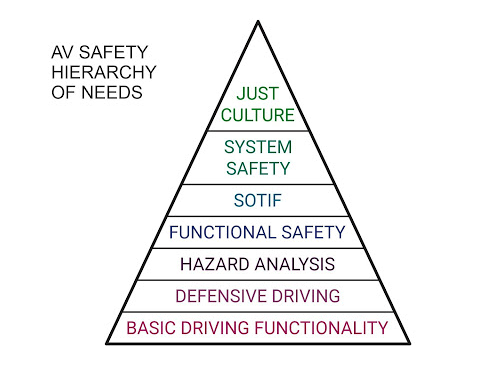
\includegraphics[width=.8\linewidth]{Figures/koopman_pyramid.png}
    \caption{Koopman's Autonomous Vehicle Safety Hierarchy of Needs~\cite{koopman}. SOTIF = safety of the intended function.}
    \label{fig:koopman_pyramid}
\end{figure}

\section{Taxonomy}
\label{taxonomy}
Our taxonomy is a software abstraction hierarchy where ``basic programming functionality'' such as code compilation and syntax checking is the lowest abstraction level,
Software architecture analysis and design is the highest abstraction level.
As we ascend the levels, just as with Koopman's pyramid in figure \ref{fig:koopman_pyramid}, 
software challenges rely more on human input and become more difficult to automate (e.g., crafting design rules vs following syntax rules).

Figure~\ref{fig:taxonomy} shows the taxonomy of autonomy levels for \cct{}.  The more abstract top levels depend on resolution of lower ones. As we move up the hierarchy, we require more human oversight of the AI; as we move down the hierarchy, rules for detecting problems are easier to formulate. Green levels are areas where \cct{} like Copilot works reasonably well, while red levels are challenging for Copilot as shown in chapters~\ref{chapter:idioms} and~\ref{chapter:smells}.

\begin{figure}[hbt!]
    \centering
    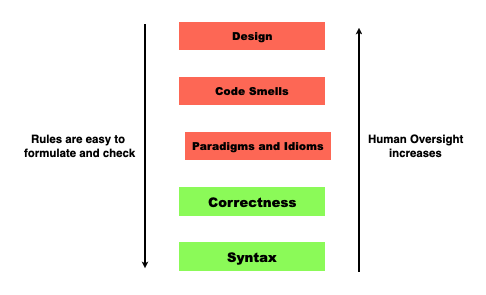
\includegraphics[width=\linewidth]{Figures/taxonomy.png}
    \caption{Hierarchy of software abstractions.}
    \label{fig:taxonomy}
\end{figure}

The challenges further up the hierarchy are nonetheless more important for software quality attributes (QA)~\cite{Ernst2017} and for a well-engineered software system.
For example, an automated solution suggested by \cct{} to the top level of the taxonomy would be able to follow heuristics to engineer a well designed software system, one which would be easy to modify and scale to sudden changes in use.
\subsection{Syntax Level}
\label{syntax}
The syntax level is the lowest abstraction level in our taxonomy. This level includes the most basic programming functionality like syntax and code compilations. This level does not require the \cct{} suggested code to successfully perform the task but to suggest code without any obvious errors like syntax errors.
For example, consider a task of perform a sorting operation on a list of numbers. To satisfy this level of abstraction, \cct{} should suggest code that is syntactically correct without any compilation errors and the code is not required to perform the sorting operation correctly. 
Figure~\ref{fig:syntax} shows the example and syntax suggestions from \cct{} at this abstraction level.

\begin{figure}[hbt!]
    \centering
    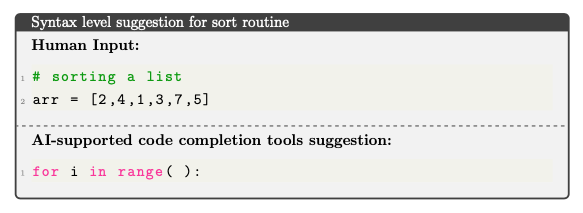
\includegraphics[width=\linewidth]{Figures/syntax.png}
    \caption{\cct{} syntax level suggestions}
    \label{fig:syntax}
\end{figure}

The goal of this software abstraction level in our taxonomy is for a \cct{} to be able to suggest code without any syntactical errors.
The capabilities required by a \cct{} to satisfy this level of abstraction are as follows:

\begin{enumerate}
    \item Suggested code should not produce any errors in code compilation.
    \item Suggested code should be syntactically correct.
\end{enumerate}

% \begin{tcolorbox}[title=Syntax level suggestion for sort routine,boxsep=.15mm]
%     %https://tex.stackexchange.com/questions/337909/tcolorbox-tcbline-style
% \textbf{Human Input:}
% \begin{lstlisting}[language={Python}]
% # sorting a list
% arr = [2,4,1,3,7,5]
% \end{lstlisting}
% \tcbline
% \textbf{\cct{} suggestion:}
% \begin{lstlisting}[language={Python}]
% for i in range( ):
% \end{lstlisting}
% \end{tcolorbox}
\section{Correctness}
\subsection{Code Smells}
The code smells level is the penultimate level of abstraction in our taxonomy, This level requires the suggested code satisfy all the previous levels of abstraction and avoid code smells in its suggestions.

For example, considering the task of  a task of perform a sorting operation on a list of numbers, to satisfy this level of abstraction, AI-supported code completion tools should
suggest a syntactically correct list sorting code, which follows the best practices like using appropriate datatype and variable to store the list.

The capabilities required by a AI-supported code completion tools to satisfy this
level of abstraction are as follows
\begin{enumerate}
    \item Satisfy requirements of syntax and correctness level.
    \item Suggest a solution that does not have any common code smells found in public code repositories.
\end{enumerate}
\subsection{Idioms}
The paradigms and idioms is the mid level of abstraction in our taxonomy. This level requires the suggested code satisfy syntax and correctness level and use common language idioms in its suggestions. 

For example, considering the task of sorting operation on a list of numbers, to satisfy this level of abstraction, \cct{} should suggest a syntactically correct list sorting code, using a well know algorithm like quick sort or bubble sort. The main goal of this level in the taxonomy is for a \cct{} to be able to use the current best practices and algorithms in its suggestions.

The capabilities required by a \cct{} to satisfy this level of abstraction are as follows
\begin{enumerate}
    \item Satisfy requirements of syntax and correctness level
    \item Use well know algorithms, best practices, and language idioms whenever possible in suggesting a solution for a problem.
\end{enumerate}
\subsection{Design}
\label{design}
The top level in our taxonomy is Design, This level requires the suggested code satisfy all the previous levels of abstractions and suggest appropriate design practices for a given input in its suggestions.

For example, considering the task of sorting operation on a list of numbers, to satisfy this level of abstraction, \cct should suggest a syntactically correct list sorting code, using a algorithm which gives the best performance for that scenario like suggesting quick sort instead of bubble sort if it is a large set of numbers. The main goal of this level in the taxonomy is for a \cct{} to be able to pick the algorithms as per given scenario in its suggestions.

\subsubsection{Design Patterns}
\label{patterns}
To satisfy design level \cct{} must be able to capture design and module level concerns. 
These include recapturing design patterns (such as Observer) and architectural tactics (such as Heartbeat) to improve and personalize suggestions. 
To do this, however, the training data must also use these patterns and best practices.
The vision is for something like Copilot to be capable of suggesting patterns like Model-View-Controller (MVC) when prompted. 

The capabilities required by a \cct{} to satisfy this level of abstraction are as follows
\begin{enumerate}
    \item Identify design and module level concerns in code files.
    \item Suggest design patterns and architectural tactics when prompted.
    \item Picking and suggesting the best applicable algorithm for a given scenario.
    \item Satisfy requirements of all previous levels of abstractions.
\end{enumerate}

% \begin{tcolorbox}[title=Code smells level suggestion for sort routine,boxsep=.15mm]
%     %https://tex.stackexchange.com/questions/337909/tcolorbox-tcbline-style
% \textbf{Human Input:}
% \begin{lstlisting}[language={Python}]
% # sorting a list
% arr = [2,4,1,3,7,5]
% \end{lstlisting}
% \tcbline
% \textbf{\cct{} suggestion:}
% \begin{lstlisting}[language={Python}, morekeywords={False, True}]
% swapped = False
% for i in range(len(arr)-1, 0, -1):
% 	for j in range(n):
% 		if arr[j] > arr[j+1]:
% 		    swapped = True
% 			arr[j], arr[j+1] = arr[j+1], arr[j]
% 	if not swapped:
% 	    break
% print(arr)
% \end{lstlisting}
% \end{tcolorbox}
\section{Chapter Summary}
